\documentclass[11pt,a4paper, final, twoside]{article}
%%%%%%%%%%%%%%%%%%%%%%%%%%%%%%%%%%%%%%%%%%%%%%%%%%%%%%%%%%%%%%%%%%%%%%%%%%%%%%%%%%%%%%%%%%%%%%%%%%%%%%%%%%%%%%%%%%%%%%%%%%%%%%%%%%%%%%%%%%%%%%%%%%%%%%%%%%%%%%%%%%%%%%%%%%%%%%%%%%%%%%%%%%%%%%%%%%%%%%%%%%%%%%%%%%%%%%%%%%%%%%%%%%%%%%%%%%%%%%%%%%%%%%%%%%%%
\usepackage{amsmath}
\usepackage{fancyhdr}
\usepackage{amsthm}
\usepackage{amsfonts}
\usepackage{amssymb}
\usepackage{amscd}
\usepackage{latexsym}
\usepackage{graphicx}
\usepackage{graphics}
\usepackage{natbib}
\usepackage[colorlinks=true, urlcolor=blue,  linkcolor=black, citecolor=black]{hyperref}
\usepackage{color}
\usepackage{natbib}
\usepackage{sectsty}
\setcounter{MaxMatrixCols}{10}


\sectionfont{\fontsize{12}{15}\selectfont}

\renewcommand{\thefootnote}{}
\setlength{\oddsidemargin}{1pt} \setlength{\evensidemargin}{1pt}
\setlength{\hoffset}{-1in} \addtolength{\hoffset}{25mm}
\setlength{\textwidth}{140mm} 
\setlength{\marginparsep}{0pt} \setlength{\marginparwidth}{0pt}
\setlength{\topmargin}{0pt}
\setlength{\voffset}{-2in} \addtolength{\voffset}{20mm}
\setlength{\textheight}{300mm}
\setlength{\headsep}{20mm}
\setlength{\footskip}{15mm}
\pagestyle{fancy}
\fancyhead{} \fancyfoot{} 



%       Theorem environments
\newtheorem{thm}{Theorem}[section]
\newtheorem{algorithm}[thm]{Algorithm}
\newtheorem{axiom}[thm]{Axiom}
\newtheorem{lem}[thm]{Lemma}
\newtheorem{example}[thm]{Example}
\newtheorem{exercise}[thm]{Exercise}
\newtheorem{notation}[thm]{Notation}
\newtheorem{problem}[thm]{Problem}
\theoremstyle{proposition}
\newtheorem{prop}{Proposition}[section]
\newtheorem{case}[thm]{Case}
\newtheorem{claim}[thm]{Claim}
\newtheorem{conclusion}[thm]{Conclusion}
\newtheorem{condition}[thm]{Condition}
\newtheorem{conjecture}[thm]{Conjecture}
\newtheorem{cor}[thm]{Corollary}
\newtheorem{criterion}[thm]{Criterion}
\theoremstyle{definition}
\newtheorem{defn}{Definition}[section]
\theoremstyle{remark}
\newtheorem{rem}{Remark}[section]
\newtheorem{solution}[thm]{Solution}
\newtheorem{summary}[thm]{Summary}
\numberwithin{equation}{section}
\renewcommand{\rmdefault}{phv} % Arial
\renewcommand{\sfdefault}{phv} % Arial
\pagenumbering{arabic} % 1, 2, 3, 4, ...

\begin{document}
\hyphenpenalty=100000


%%%%%%%%%%%%%%%
%% MY MACROS %%
%%%%%%%%%%%%%%%

\newcommand{\R}{\mathbb{R}}
\newcommand{\m}{\mathsf}
\newcommand{\lap}{\Delta}
\newcommand{\tp}{^\intercal}
\newcommand{\mesh}{\mathcal{M}}

\begin{center}

{\Large \textbf{\\Solving PDEs on Deconstructed Domains\\for Geometry Processing}}\\[5mm]
{\large \textbf{Herng Yi Cheng, Mitchell Dembowski, \\Silvia Gonz\'alez Sell\'an and Christine Ma }\\[1mm]}
{\normalsize \emph{Under the supervision of Professor Alec Jacobson}\\[1mm]}
\end{center}

\section{Introduction}

The Laplace equation and Possion equation are partial differential equations (PDEs) which arise naturally from analyzing heat flow, Maxwell's equations of electromagnetism, and shape recognition in computer graphics \cite{ShapeRepresentation}. We studied a new way to solve these equations on overlapping triangular mesh domains, in order to smoothen the computer animation of objects that are represented using those meshes. We designed several variants of a divide-and-conquer solution method, and tested them against each other for accuracy.

\section{Background}\label{I1}

%We studied a new way to solve some partial differential equations (PDEs) using a divide-and-conquer method. In particular, we studied
The Laplace equation models the steady-state distribution of heat on a domain $A \subset \R^2$ with each point $(p_1,p_2)$ on its boundary $\partial A$ held at a fixed temperature $g(p_1,p_2)$. The steady-state temperature distribution $u(x,y) : A \to \R$ must satisfy
\begin{align}
\lap u (x,y) &= 0 &\text{ for all } &(x,y) \in A\setminus\partial A,\label{Eq:LaplaceEquation}\\
u(p_1,p_2) &= g(p_1,p_2) &\text{ for all } &(p_1,p_2) \in \partial A\label{Eq:BoundaryCondition},
\end{align}
where \eqref{Eq:LaplaceEquation} is the Laplace equation, $\lap = \frac{\partial^2}{\partial x^2} + \frac{\partial^2}{\partial y^2}$ is the Laplace operator and \eqref{Eq:BoundaryCondition} is the boundary condition. \eqref{Eq:LaplaceEquation} can be generalized to the Poisson equation
\begin{equation}
\lap u = h \text{ for constant } h \in \R.
\end{equation}

The usual method for solving these PDEs numerically, known as finite element discretization, consists in approximating $A$ using a triangle mesh with vertices $v_1,\dotsc,v_n$ and substituting every function $f$ defined on $A$ by the vector of its finite evaluations $f_i=f(v_i)$. From this discrete perspective, solving either of the equations above becomes an optimization problem over a finite number of variables. The solutions to these optimization problems approximate the smooth solutions of the original PDE.

%To solve these PDEs numerically, these equations that involve ``smooth'' differentiation over a continuous space are often ``discretized'' by approximating $A$ using a triangle mesh with vertices $v_1,\dotsc,v_n$, and formulating a ``dual optimization problem'' to the PDE over a finite number of variables. The solutions of these optimization problems approximate smooth solutions of the original PDEs.

In the case of the Laplace and Poisson equations, this optimization problem amounts to minimizing the discrete Dirichlet energy function, which has the form
%The optimization problem consists in minimizing the Dirichlet energy function, which has the form
\begin{equation}\label{Eq:DirichletEnergy}
E(u) = \frac12\m{u}_A\tp\m{Q}\m{u}_A + \m{c}\tp\m{u}_A \text{, where } \m{u}_A = \begin{bmatrix}
u(v_1) \\ \vdots \\ u(v_n)
\end{bmatrix},
\end{equation}
for some constant vector $\m{c} \in \R^n$. The $n \times n$ cotangent matrix $\m{Q}$ is ubiquitous in geometry processing and serves as the discrete equivalent of the continuous Laplace operator seen above; its derivation can be found in \cite{AlecThesis}. This energy is to be minimized over all $\m{u}_A \in \R^n$, subject to the boundary condition that fixes the entries of $\m{u}_A$ that correspond to vertices on $\partial A$. Expanding the matrix products in \eqref{Eq:DirichletEnergy} shows that the right-hand-side is quadratic in the entries of $\m{u}_A$, therefore standard techniques of quadratic programming that minimize quadratic functions subject to constraints yield the energy minimizer, or the vector $\m{u}_A$ that minimizes \eqref{Eq:DirichletEnergy}. However, the precise method by which these optimization problems are solved will not be a concern  throughout the paper.


%\section{Introduction}


\newpage
\section{Domain Decomposition}

How well the energy minimizers approximate solutions to the smooth PDEs depends on the quality of the mesh. Two important parameters of a mesh that determine its quality are its coarseness, as measured by the average lengths of edges (segments connecting vertices), and its regularity, as measured by the aspect ratios of its triangles. Very regular meshes have triangles that are roughly equilateral, while long and thin triangles make an irregular mesh. As mesh quality improves, the energy minimizers should converge to solutions to the PDEs.

Generating quality meshes that represent complex shapes is an active field of research. In 3D, it is often much easier to decompose complex 3D shapes into the union of simpler domains, and then generate quality meshes for those domains. Thus, we study a divide-and-conquer approach to minimize the Dirichlet energy over the union of many domains by minimizing parts of that energy over each individual domain, while demanding that the minimizers agree wherever the domains overlap, to ensure a compatible combined minimizer. We will refer to this as the consistency requirement (formalized below). We implemented this approach to handle general pairs of overlapping 2D domains $A$ and $B$, with corresponding meshes.

However, functions over $A$ and $B$ cannot be compared because they are represented, respectively, by vectors $\m{u}_A$ and $\m{u}_B$, whose entries are values on different sets of vertices. In order to formulate that consistency requirement, we linearly interpolate from $\m{u}_A$ over the triangles of $A$'s mesh to reconstruct a function $u_A : A \to \R$; this is to say, we take $u_A$ to be the only function which is linear on every triangle of $A$'s mesh while taking the values of $\m{u}_A$ at its vertices.
Similarly, we reconstruct $u_B : B \to \R$. This reconstruction can be plotted out, as in Figure~\ref{Fig:VisualizingConstraints}. Our contribution is to analyze the following two formulations of the consistency requirement as the linear constraints of quadratic programs, in the hopes that they can be generalized to 3D.
\begin{description}
  \item[Overlap sampling constraint (OSC)] $u_A$ and $u_B$ must agree at the combined vertices of both meshes.
  \item[Dirichlet sampling constraint (DSC)] $u_A$ and $u_B$ must agree at the vertices of both meshes that lie on $\partial(A \cap B)$ (a small subset of the overlap sampling constraint).
\end{description}

\begin{figure}[h]\centering
\begin{tabular}{ccc}\\
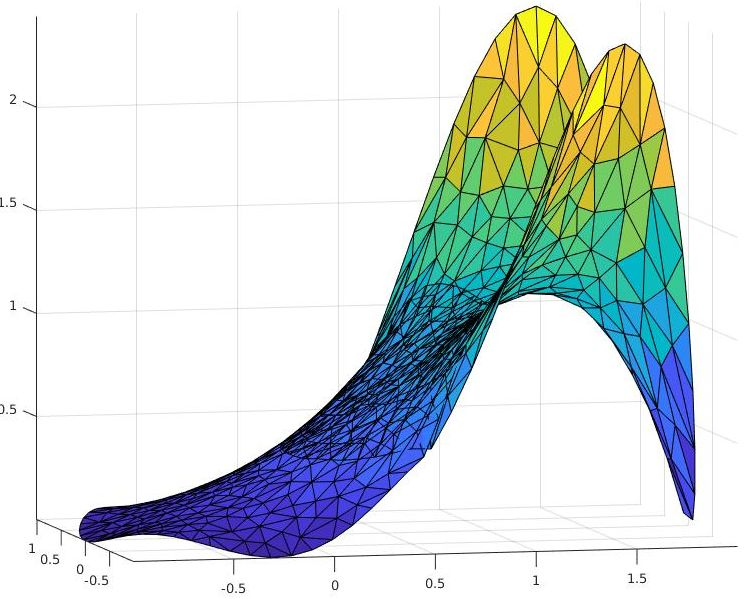
\includegraphics[height=5cm]{Overlap_sampling_constraint} & \quad &
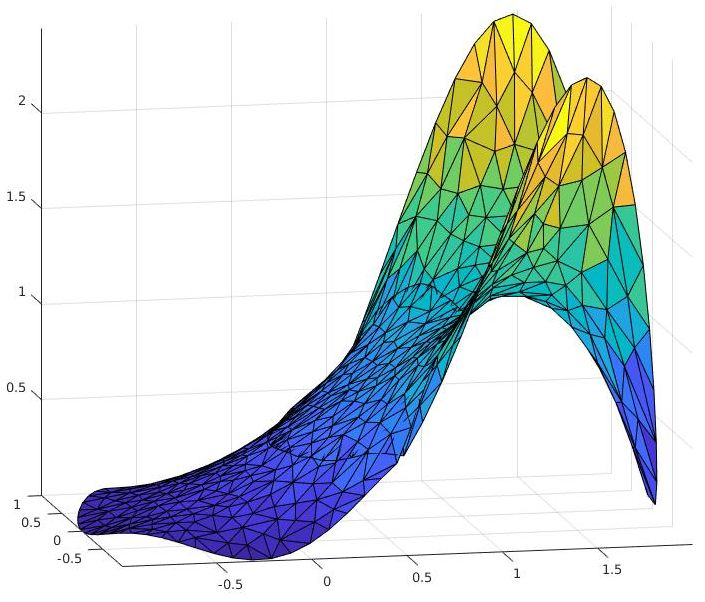
\includegraphics[height=5cm]{Dirichlet_Sampling_Constraint}
\end{tabular}
\caption{Energy minimizers for the OSC (left) and the DSC (right), subject to the same boundary condition $g(x,y) = (x+0.3)^2y^2$. Note how the two generate virtually identical solutions, even though the second one is only enforcing equality on a much smaller number of vertices.
}
%The Dirichlet sampling constraint yields two barely-distinguishable layers over $A \cap B$, where equality is not enforced.}
\label{Fig:VisualizingConstraints}
\end{figure}

\newpage
\section{Experiments and results}\label{I2}

From each constraint we derived a quadratic program to solve the Laplace or Poisson equation over $A \cup B$, subject to a boundary condition $g : \partial(A \cup B) \to \R$. Namely, we minimized a weighted combination of $E(u_A)$ and $E(u_B)$, such that $u_A$ and $u_B$ satisfy that constraint, and take values on vertices in $\partial(A \cup B)$ as dictated by $g$. We subjected each type of quadratic program to a  convergence test over two annular domains with annular union (see figure \ref{Fig:AnnulusShape}), and measured the maximum of the distance of the approximations provided by each method to the known analytical solution. We repeated this test for $\lap u=0$, $\lap u=1$ and for different levels of mesh regularity. $\lap u = 1$ was chosen for a simple nonzero right-hand side; using any other nonzero constant would have simply scaled $u$.

We concurrently tested the ``ideal'' method: combining the meshes of $A$ and $B$ into a combined mesh for $A \cup B$, and treating the minimizer of the Dirichlet energy over that combined mesh as a ground truth (GT) proxy to the analytic solution, when the latter is unknown. This ground truth would be unavailable in 3D where combining meshes is far more difficult, but it serves as a useful benchmark of our quadratic programs in 2D.

\begin{figure}[h]
\begin{center}
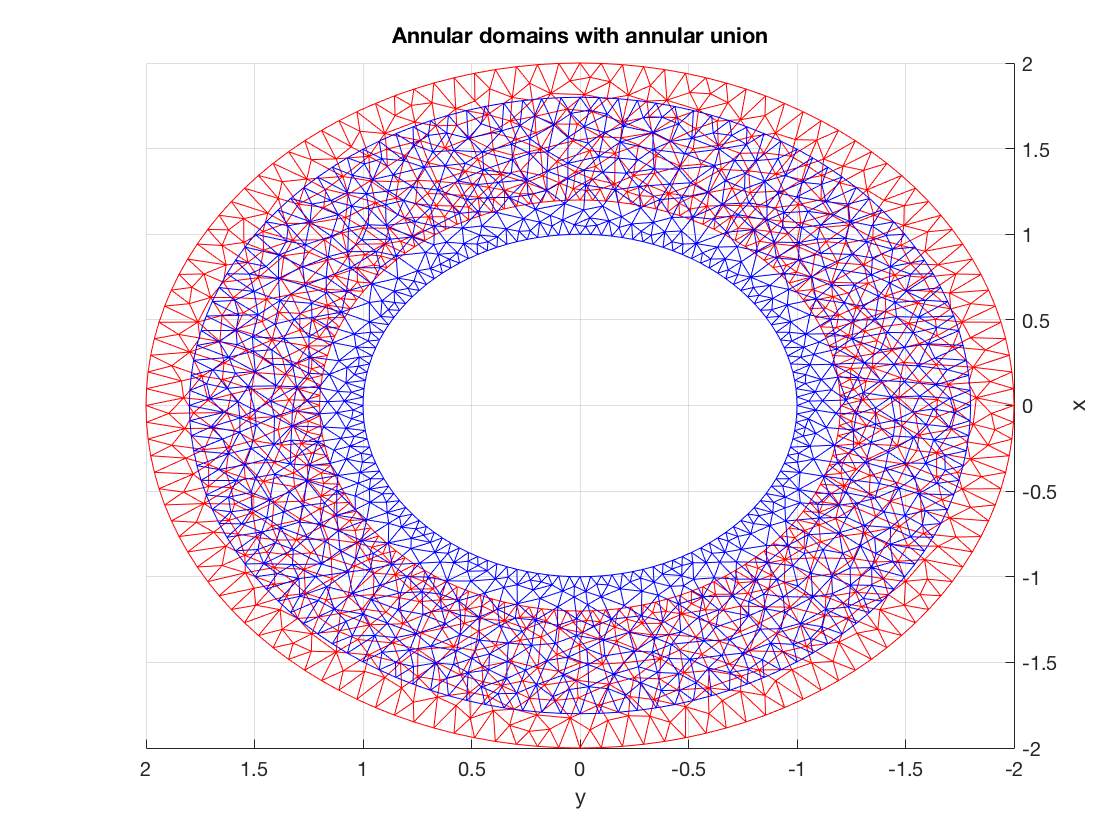
\includegraphics[width=0.6\textwidth]{annulusshape.png}
 \caption{A pair of annular domains, in blue and red.}
\label{Fig:AnnulusShape}
\end{center}
\end{figure}

Our results, presented in Figure \ref{Fig:AnnulusResults}, show the Dirichlet sampling constraint to be clearly superior. While the overlap constraint appears to be accurate when solving $\lap u=0$ on regular meshes, it fails and does not even converge to the analytical solution for $\lap u = 1$, or when the meshes become increasingly irregular. As expected, the ground truth deviates the least from the analytic solution and converges to it the fastest.

We performed similar tests on different domain shapes, which can be seen in Figure~\ref{Fig:ExamplesShape}. Since no analytical solution is available for these pairs of meshes, we simply measured the error between our methods and the co-refined ground truth (yellow line in figure~\ref{Fig:AnnulusResults}), safely assuming that this last one will surely converge to the smooth solution of the PDE. The results obtained from these experiments agreed completely with those observed for the pair of annular domains.

\newpage

\begin{figure}[h]
\begin{center}
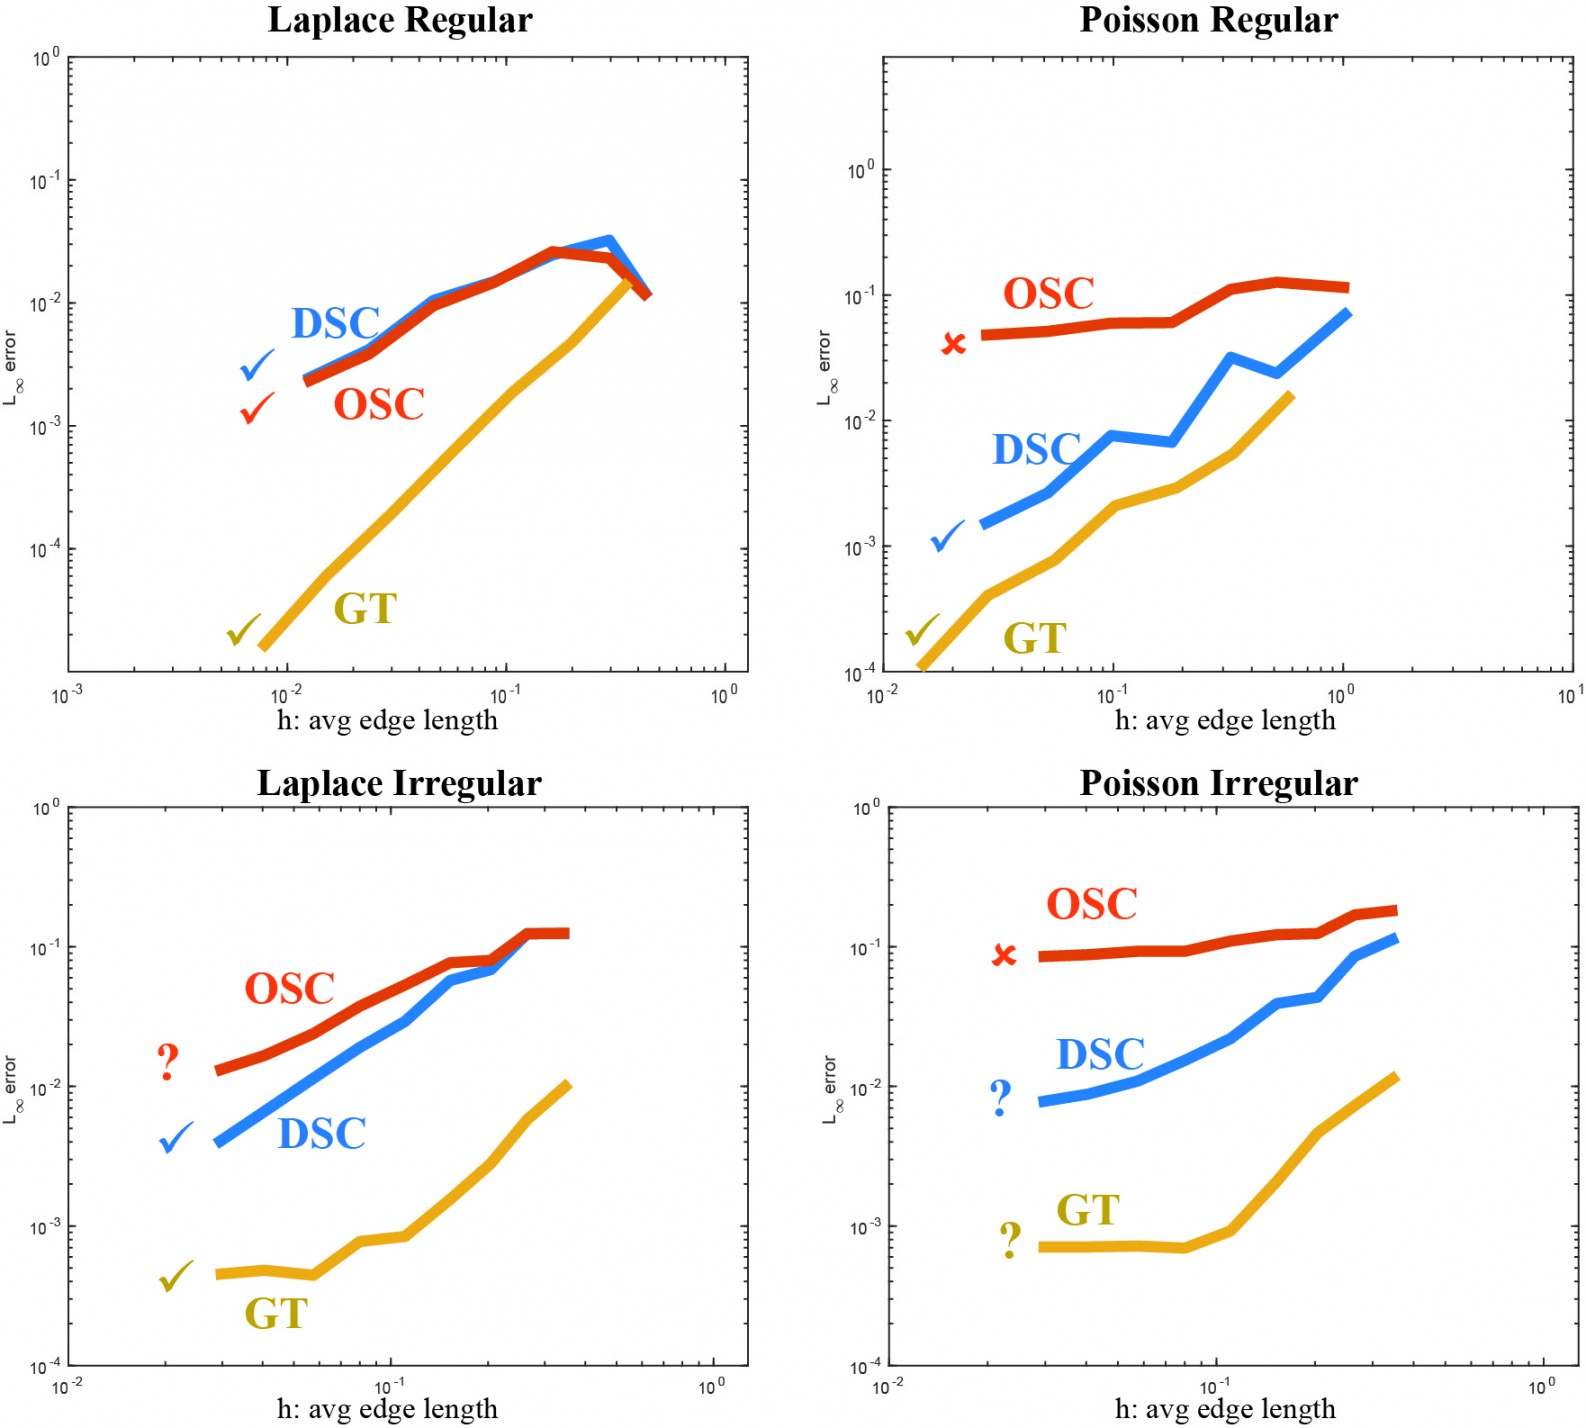
\includegraphics[width=.95\textwidth]{allfigs2.jpg}
\caption{Convergence of our methods for annular domains. The top row shows the results for regular meshes, while the bottom one shows the results for irregular meshes. The left column contains results for the equation $\lap u=0$, while the right one does so for $\lap u=1$.}
\label{Fig:AnnulusResults}
\end{center}
\end{figure}



\begin{figure}[h]
\begin{center}
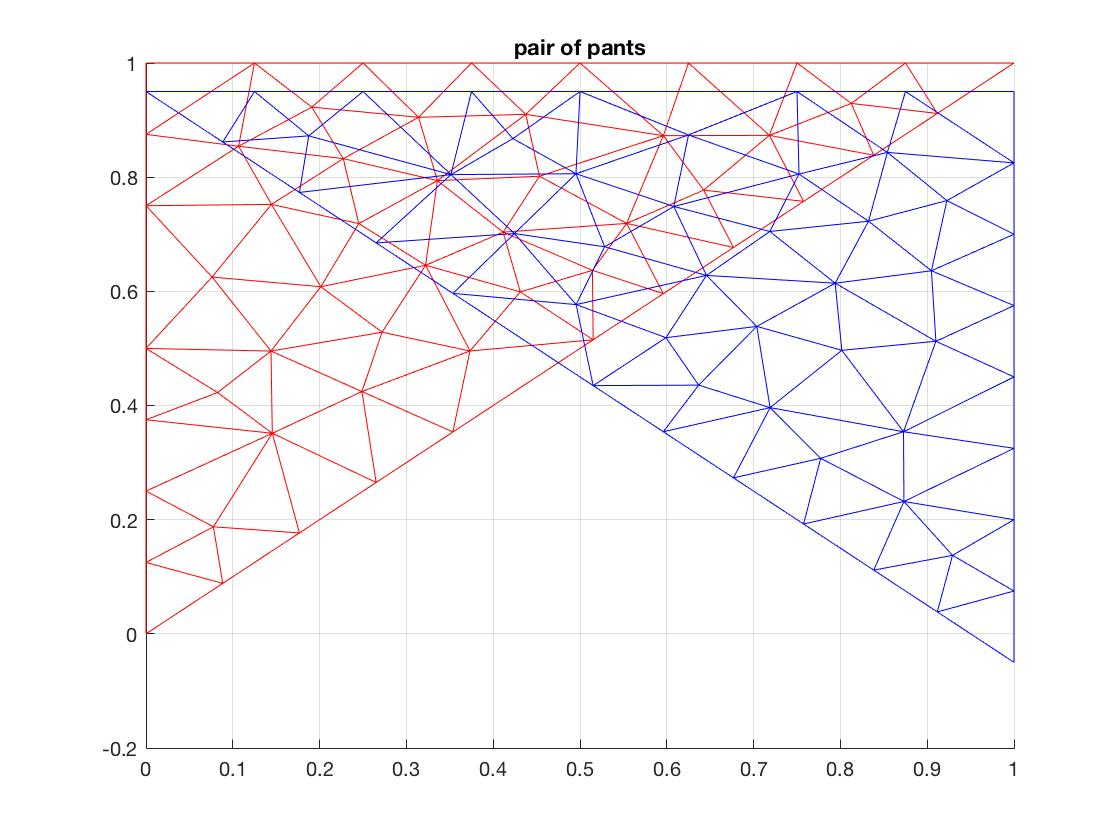
\includegraphics[width=0.3\textwidth]{pres1.jpg} \quad
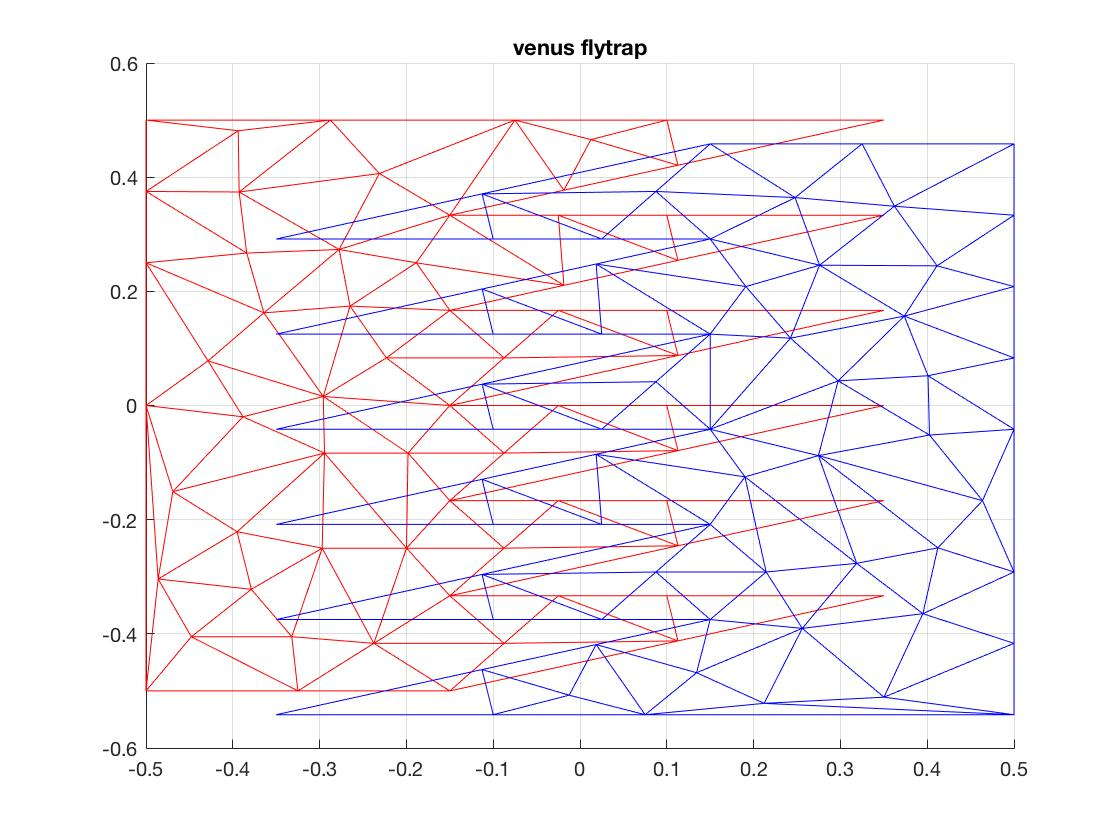
\includegraphics[width=0.3\textwidth]{pres2.jpg} \quad
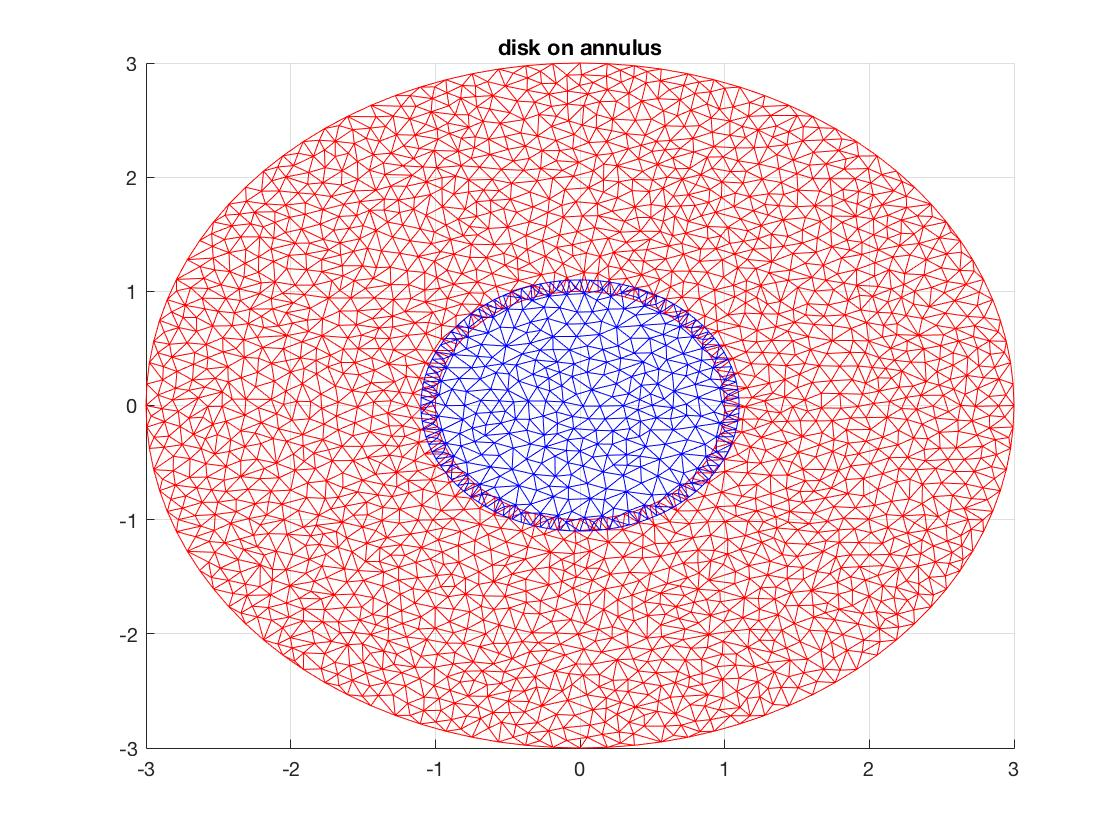
\includegraphics[width=0.3\textwidth]{pres3.jpg} \\
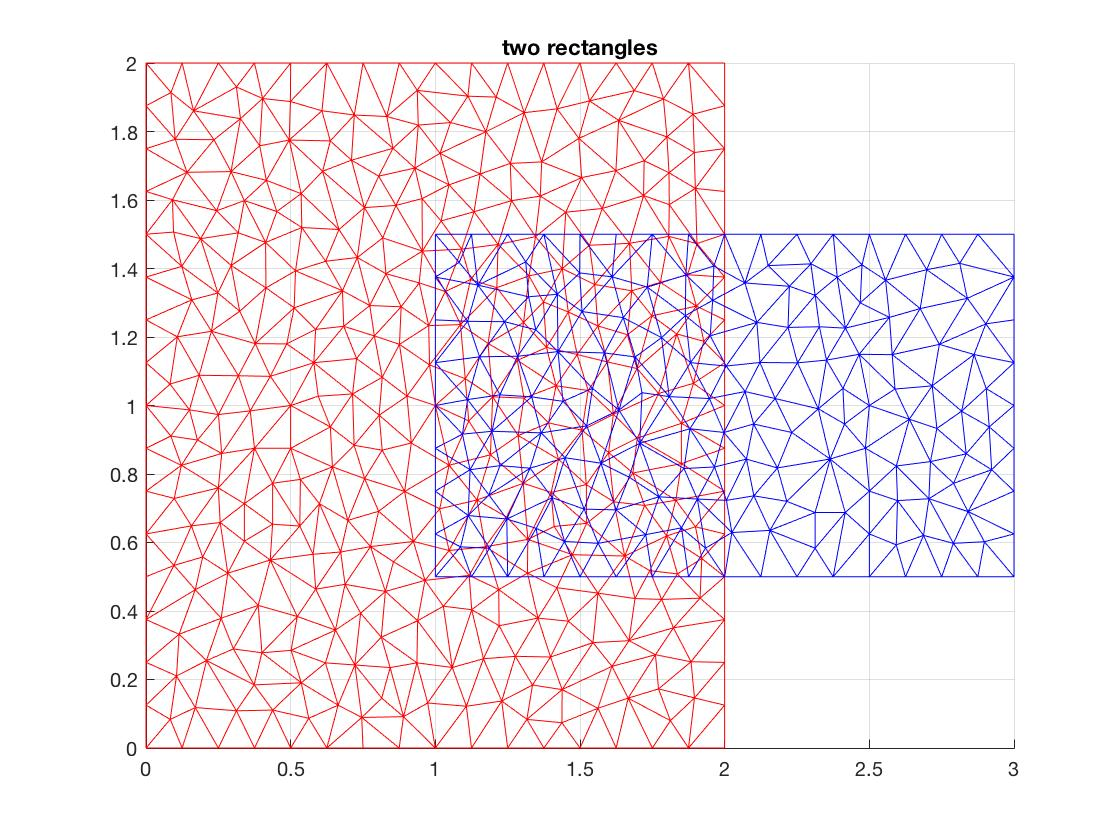
\includegraphics[width=0.3\textwidth]{pres5.jpg} \quad
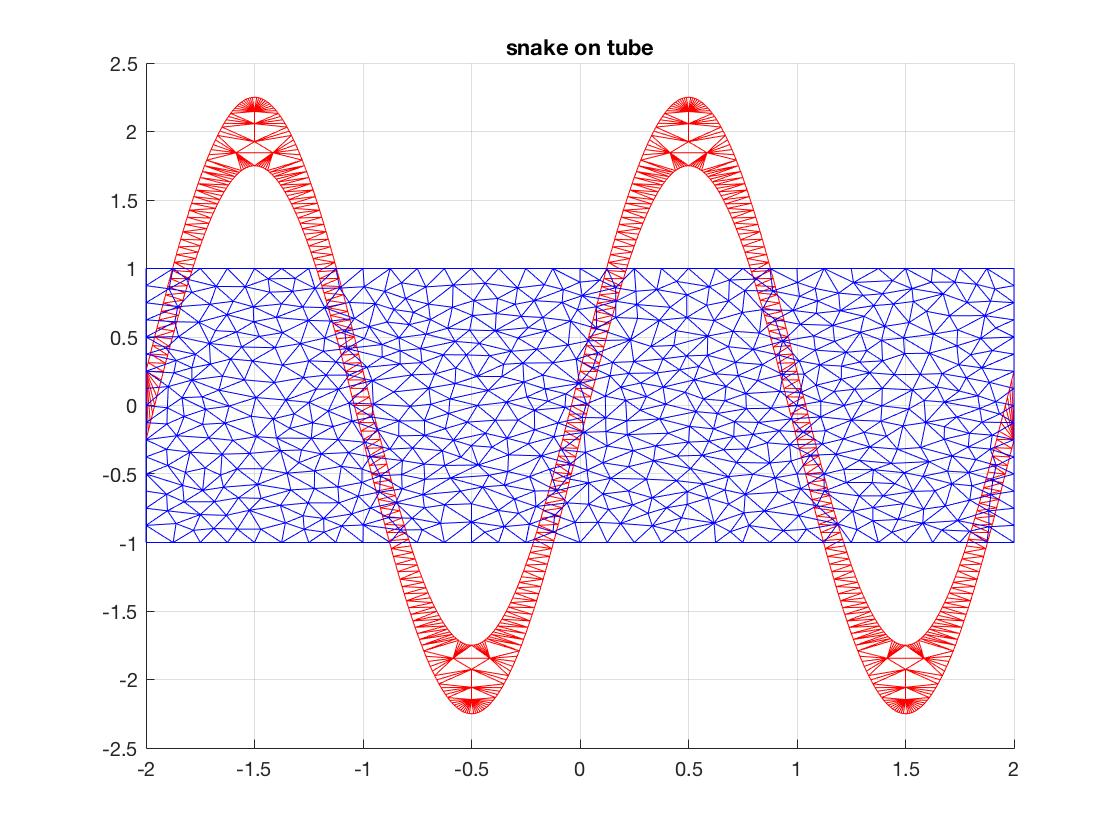
\includegraphics[width=0.3\textwidth]{pres6.jpg} \quad
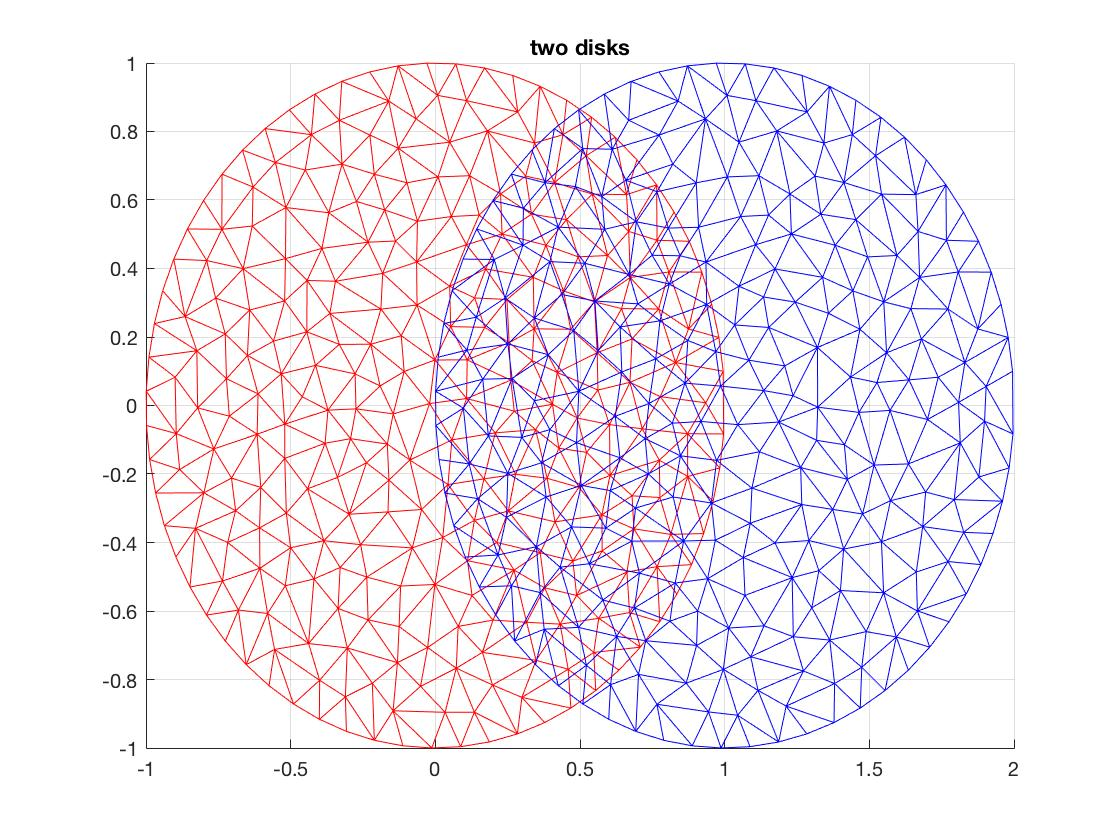
\includegraphics[width=0.3\textwidth]{pres7.jpg}
\caption{Examples of pairs of meshes over which we have tested convergence.}
\label{Fig:ExamplesShape}
\end{center}
\end{figure}

\newpage
\section{Conclusion}

The overlap sampling constraint performed inconsistently between $\lap u = 0$ and $\lap u = 1$, as well as between regular and irregular meshes, although it was surprisingly accurate when solving the Laplace equation on regular meshes.

The Dirichlet sampling constraint converged in every one of our experiments for both the Laplace and Poisson equations, regardless of regularity and shape of the meshes. While converging slower than the ground truth, its rate of convergence appears to be at least linear. It is the best candidate for future research to generalize to 3D, progressing toward our goal of solving PDEs over the union of multiple domains when computing a common mesh is infeasible.

\mbox{}\\

\noindent {\Large\textbf{Acknowledgement}\\[1mm] }

The authors would like to thank Prof. Alec Jacobson for his patient and dedicated mentorship, as well as the Fields Institute for bringing our research group together, and supporting our research with a stipend, through the Fields Undergraduate Summer Research Program. The third author would also like to express deep gratitude to the Mar\'ia Cristina Masav\'eu Peterson Foundation for its financial support of her studies.

\bibliography{Bibliography}
\bibliographystyle{plain}

\end{document}

